\item Cada uma das três bolas tem uma massa $m$. Se $A$ tem uma velocidade $v$ imediatamente antes da colisão direta com $B$, determine a velocidade de $C$ após a colisão. O coeficiente de restituição entre cada bola é $e$. Despreze
a dimensão de cada bola.

\import{sections/answers/}{answer-5}

\vspace{-1.4cm}
\begin{flushright}
	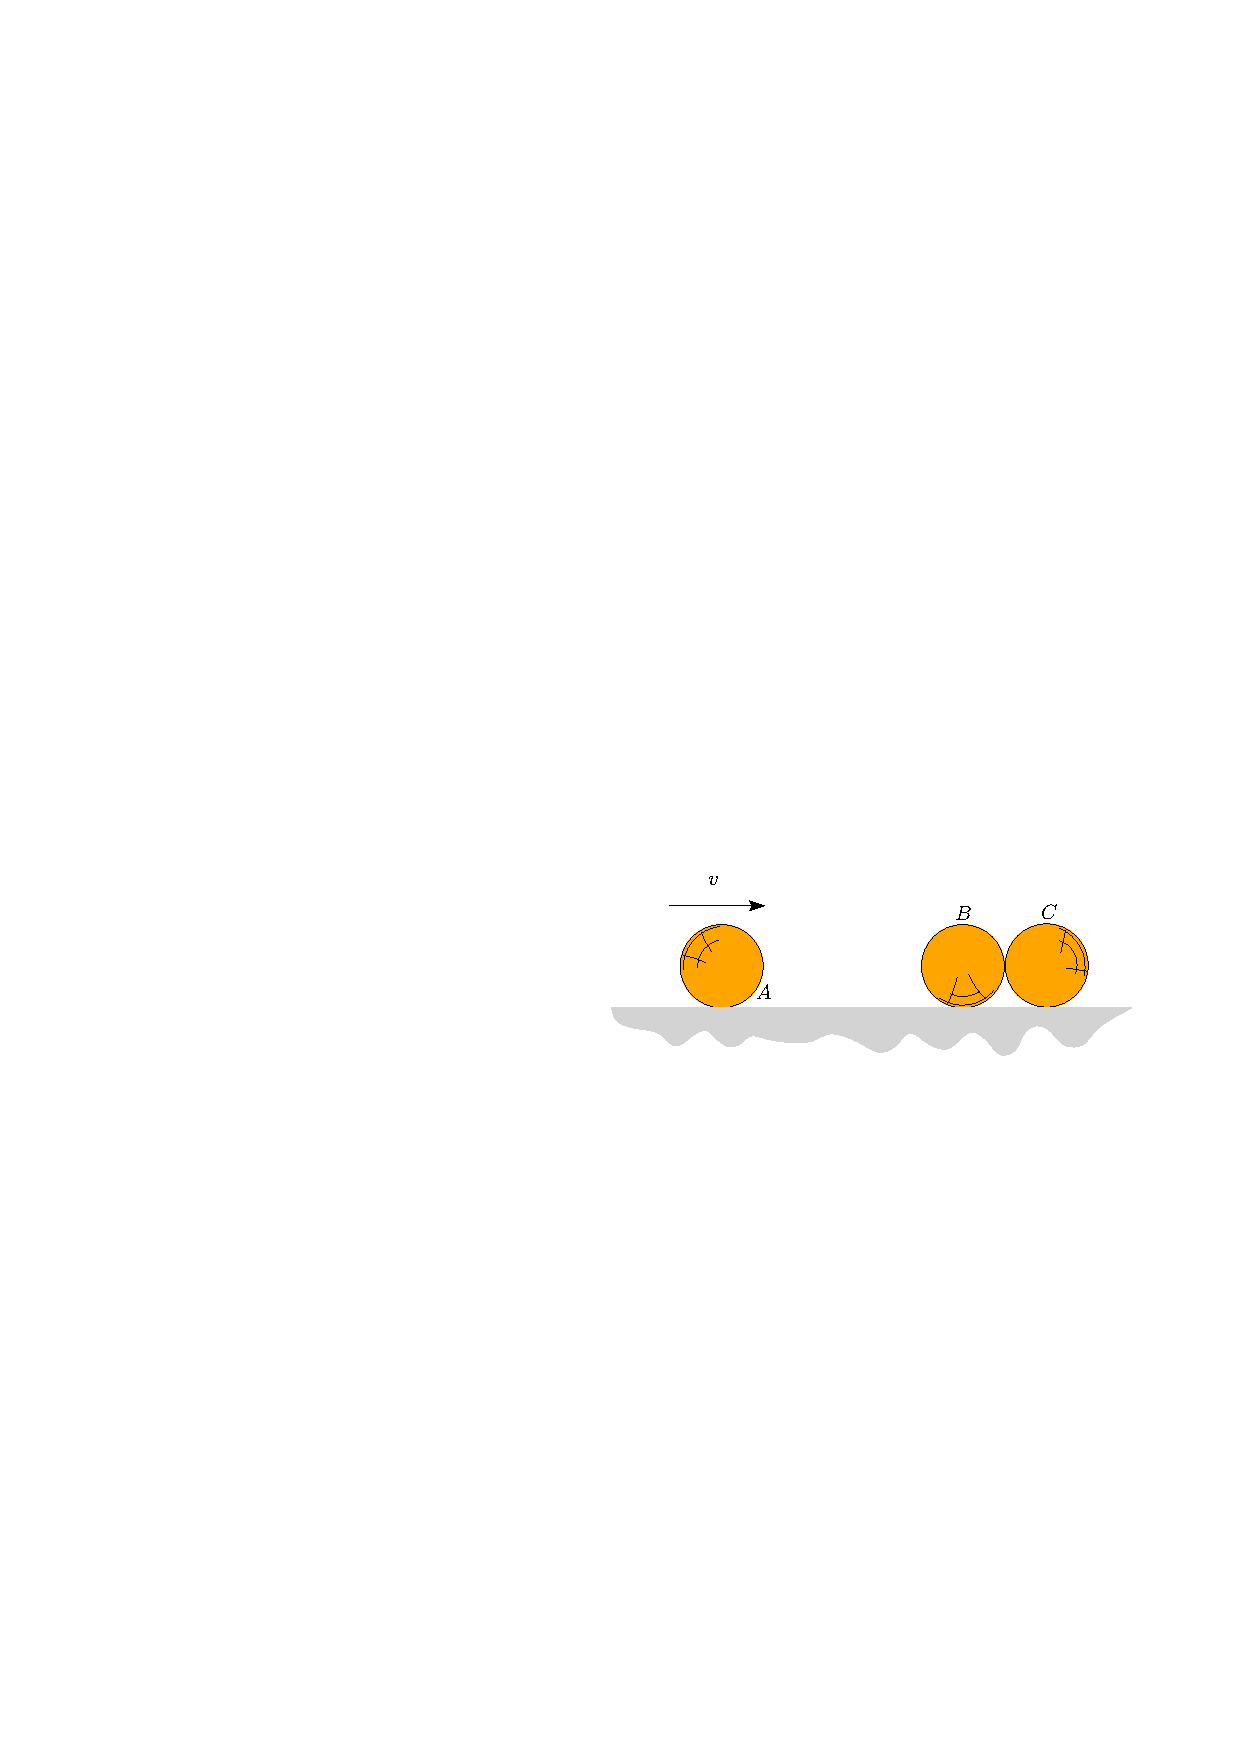
\includegraphics[scale=1.2]{images/draw_5}
\end{flushright}